% ****** Start of file sorsamp.tex ******
%
%   This file is part of the AIP files in the AIP distribution for REVTeX 4.
%   Version 4.2a of REVTeX, December 2014
%
%   Copyright (c) 2014 American Institute of Physics.
%
%   See the AIP README file for restrictions and more information.
%
% TeX'ing this file requires that you have AMS-LaTeX 2.0 installed
% as well as the rest of the prerequisites for REVTeX 4.2
%
% It also requires running BibTeX. The commands are as follows:
%
%  1)  latex  sorsamp
%  2)  bibtex sorsamp
%  3)  latex  sorsamp
%  4)  latex  sorsamp
%
% Use this file as a source of example code for your aip document.
% Use the file aiptemplate.tex as a template for your document.
\documentclass[%
 sor,
%aip,
%twoside,
%groupedaddress,
%jmp,
 jor,
 amsmath,amssymb,
%preprint,%
 reprint,%
%author-year,%
%author-numerical,%
]{revtex4-2}

\usepackage{graphicx}% Include figure files
\usepackage{dcolumn}% Align table columns on decimal point
\usepackage{bm}% bold math
%\usepackage[mathlines]{lineno}% Enable numbering of text and display math
%\linenumbers\relax % Commence numbering lines
\usepackage{hyperref}
\usepackage{subfig}
\usepackage{float}

\usepackage[percent]{overpic}  % en el preámbulo


\begin{document}

\preprint{AIP/123-QED}

\title[Stochastic Evolutionary Game Theory]{Stochastic Evolutionary Game Theory}% Force line breaks with \\

\author{Ali-Salem Amari}
 \email{alisalemstd@correo.ugr.es}
\author{Ana Rodríguez Garrido}
 \email{anagarrido12@correo.ugr.es}

\date{\today}% It is always \today, today,
             %  but any date may be explicitly specified

\begin{abstract}
Este trabajo analiza estrategias evolutivas en poblaciones finitas mediante una dinámica estocástica de tipo nacimiento-muerte, utilizando el proceso de Moran y la función de Fermi. Se calculan la probabilidad y el tiempo medio de fijación de un mutante, y se conecta esta dinámica con la ecuación del replicador. Se estudian tanto el régimen estocástico como el determinista, identificando los cuatro escenarios evolutivos clásicos. El análisis se extiende a ambientes fluctuantes, donde se explora el dilema entre estrategias especializadas y generalistas, mostrando que el ritmo de cambio ambiental puede favorecer comportamientos más arriesgados. Finalmente, se aplica este marco a tumores, mostrando cómo las interacciones celulares guían la evolución y sugiriendo terapias que modifiquen el entorno en lugar de atacar directamente las células cancerosas.
\end{abstract}


\maketitle

\section{\label{sec:level1}Introducción}

A principios del siglo XX John von Neumann desarrolló una rama matemática en la que pretendía analizar las decisiones estratégicas en contextos de interacción entre múltiples agentes racionales. 
Von Neumann definió la teoría de juegos clásica como ``una teoría que trata de la determinación de estrategias óptimas en los juegos competitivos, donde el resultado para cada jugador depende de las elecciones de todos los participantes" \cite{vonNeumann1944}. 

Por su parte, la teoría de juegos evolutiva aboga por el estudio de estrategias que conducen a un mayor éxito en la interacción dentro de una población que tienden a prevalecer, ya sea por capacidad reproductiva o por imitación de comportamientos exitosos, sin asumir racionalidad ni toma de decisiones consciente: 
``la teoría de juegos evolutiva es la aplicación de la teoría de juegos a poblaciones en evolución dentro de la biología. Define un marco de competencias, estrategias y herramientas analíticas mediante el cual puede modelarse la competencia darwiniana" \cite{MaynardSmith1982}. \newline


La piedra angular de las interacciones entre agentes es la matriz de pagos, que define el beneficio que recibe cada agente al enfrentar distintas combinaciones de estrategias:
\begin{equation}
M =
\begin{bmatrix}
a & b \\
c & d
\end{bmatrix}
\end{equation}

El valor \(a\) representa la ganancia obtenida por un jugador que utiliza la estrategia \(A\) al enfrentarse a otro jugador que también usa \(A\); \(b\) es la ganancia de \(A\) cuando juega contra un jugador que emplea la estrategia \(B\); \(c\) corresponde a la ganancia de \(B\) al enfrentarse a un jugador con estrategia \(A\); y finalmente, \(d\) es la ganancia que recibe un jugador con estrategia \(B\) al jugar contra otro jugador que también utiliza \(B\), \cite{Arne}.
\\

Para analizar cómo evolucionan las estrategias dentro de una población se usa tanto la dinámica del replicador como la dinámica estocástica, para relacionar ambas es fundamental considerar el límite de grandes poblaciones para recuperar la dinámica determinista.

\section{\label{sec:level2}Dinámica evolutiva estocástica}
\label{defpaymed}

Consideramos un sistema de \(N\) individuos en el que todos interactúan entre sí. Supongamos que \(j\) de ellos adoptan la estrategia \(A\) y los \(N - j\) restantes la estrategia \(B\).
La probabilidad de seleccionar al azar un par formado por un individuo con estrategia \(A\) y otro con estrategia \(B\) es \(\frac{j(N - j)}{N^2}\). Para modelar la probabilidad de que un individuo adopte la estrategia de otro, se emplea una regla estocástica basada en la distribución de Fermi, la cual depende de la diferencia de pagos \(\Delta \pi=\pi_A-\pi_B\) entre estrategias. El pago total que recibe un individuo con estrategia \(A\) y otro con estrategia \(B\) es respectivamente: \(\pi_A(j) = \frac{j - 1}{N} a + \frac{N - j}{N} b\) y  
\(\pi_B(j) = \frac{j}{N} c + \frac{N - j - 1}{N} d\) \cite{Ruben}.

\begin{itemize}
    \item La probabilidad de que un individuo con estrategia \(B\) adopte la estrategia \(A\) (i.e. \(j \rightarrow j+ 1\)): $T_j^+ = \frac{j(N - j)}{N^2} \cdot \frac{1}{1 + \exp(-w \Delta \pi)}$
    

    \item La probabilidad de que un individuo con estrategia \(A\) adopte la estrategia \(B\) (i.e. \(j \rightarrow j - 1\)): $T_j^- = \frac{j(N - j)}{N^2} \cdot \frac{1}{1 + \exp(w \Delta \pi)}$
    
\end{itemize}

Se derivan los conceptos de probabilidad de fijación  y tiempo de fijación de un mutante para entender su posible impacto evolutivo en una población finita con estados absorbentes $j=0;j=N$, \cite{Arne}. 

\begin{equation}
    \text{Probabilidad de fijacion de un mutante \hspace{0,1 cm}}\phi_1=\frac{1}{\left(1+\sum_{m=1}^{N-1}\prod_{j=1}^{m}\xi_j \right)}
\end{equation}

\begin{equation}
   \text{Tiempo de fijacion de un mutante \hspace{0,1 cm}} t_1=\phi_1 \left( \sum_{w=1}^{N-1}\sum_{l=1}^{w}\frac{1}{T_l^+}\prod_{m=l+1}^{w}\xi_m \right )
\end{equation}

Todo el desarrollo matemático se encuentra en el Apéndice \ref{ApendiceA}.

\subsection{Interpretación de la dinámica nacimiento-muerte}

Partiendo de la dinámica estocástica definida por las probabilidades de transición \(T_j^\pm\), es posible interpretar el proceso como una dinámica de nacimiento muerte en tiempo discreto para la frecuencia \(x=j/N\) de la estrategia \(A\). Esta interpretación permite aplicar el formalismo de la ecuación maestra y, mediante la expansión de Kramers-Moyal, aproximar la dinámica por una ecuación de Langevin considerando el término de deriva \(A(x)\) y de difusión \(B(x)\), \cite{CalvoTema3}.

\begin{equation}
    \dot{x}(t)=A(x)+\sqrt{B(x)} \xi(t) \Rightarrow \dot{x}(t)=(T_x^+-T_x^-)+\sqrt{\frac{(T_x^++T_x^-)}{N}}\xi(t)
\end{equation}

Tomando el límite $N \xrightarrow{} \infty$ se recupera la dinámica del replicador, con  \(\pi_A(x)=(x-\frac{1}{N})a+(1-x)b \xrightarrow{N\xrightarrow{}\infty}ax + (1 - x)b\) y \(\pi_B(x)=xc+(1-x-\frac{1}{N})d \xrightarrow{N\xrightarrow{}\infty}cx + (1 - x)d \).

\begin{equation}
\dot{x}(t)=x(1-x)\text{tanh}\left(+\frac{w}{2} \Delta \pi(x)\right)=x(1-x)\text{tanh}\left(+\frac{w}{2} \left[\pi_A(x)-\pi_B(x)\right] \right)    
\end{equation}

Todo el desarrollo matemático se encuentra en el Apéndice \ref{ApendiceB}.

\subsection{Estabilidad de los puntos fijos}
\label{estabilidad}

Consideramos el sistema $\dot{x}(t)=x(1-x)\text{tanh}(+\frac{w}{2}(\alpha x+\delta))$, siendo \(\alpha =(a-b-c+d), \delta=(b-d)\). Los puntos fijos $x^*$ se encuentran resolviendo la ecuación $\dot{x}=0$:

\[
x^*=0,x^*=1 \text{\hspace{0,1 cm}o\hspace{0,1 cm}} \text{tanh}(+\frac{w}{2} (\alpha x+\delta)))=0 \Leftrightarrow \alpha x +\delta=0 \Rightarrow x^*=\frac{-\delta}{\alpha}=\frac{d-b}{a-b-c+d} \in (0,1)
\]


La estabilidad se puede analizar a través de $f'(x^*)$, se calcula la derivada $f'(x)=(1-2x)\text{tanh}(\frac{w}{2}(\alpha x +\delta))+x(1-x)\text{sech}^2(\frac{w}{2}(\alpha x +\delta))\frac{\alpha w}{2}$ y se evalúan los puntos fijos $x^*$, \cite{CalvoTema2}.

\begin{itemize}
    \item Para \( x^* = 0 \): \( f'(0) =\text{tanh}(\frac{w}{2}\delta)=\text{tanh}(\frac{w}{2}(b-d))\)

    Si $b>d \Rightarrow f'(0)>0 \Rightarrow \text{Inestable}$\\
    Si $b<d \Rightarrow f'(0)<0 \Rightarrow \text{Estable}$

     \item Para \( x^* = 1 \): \( f'(1) =-\text{tanh}(\frac{w}{2}(\alpha +\delta))=-\text{tanh}(\frac{w}{2}(a-c))\)

    Si $a>c \Rightarrow f'(1)<0 \Rightarrow \text{Estable}$\\
    Si $a<c \Rightarrow f'(1)>0 \Rightarrow \text{Inestable}$

    \item Para \( x^* = \frac{-\delta}{\alpha} \): \( f'(\frac{-\delta}{\alpha}) =x^*(1-x^*)\frac{\alpha w}{2}\), como \(x^*=\frac{-\delta}{\alpha} \in (0,1) \Rightarrow x^*(1-x^*) >0\)

    Si $\alpha>0 \Rightarrow (a>c,d>b) \Rightarrow  f'(\frac{-\delta}{\alpha})>0 \Rightarrow \text{Inestable}$\\
    Si $\alpha<0 \Rightarrow (a<c,d<b) \Rightarrow f'(\frac{-\delta}{\alpha})<0 \Rightarrow \text{Estable}$\\
   
\end{itemize}

Si se compara con la ecuación del replicador usual \(\dot{x}(t)=x(1-x)(\alpha x+\delta)\), se encuentran los mismos puntos fijos. La estabilidad se puede analizar a través de $f'(x^*)$, se calcula la derivada $f'(x)=(1-2x)(\alpha x+\delta)+x(1-x)\alpha$ y se evalúan los puntos fijos $x^*$, \cite{CalvoTema2}.

\begin{itemize}
    \item Para \( x^* = 0 \): \( f'(0) =\delta=b-d\)

    Si $b>d \Rightarrow f'(0)>0 \Rightarrow \text{Inestable}$\\
    Si $b<d \Rightarrow f'(0)<0 \Rightarrow \text{Estable}$

     \item Para \( x^* = 1 \): \( f'(1) =-(\alpha +\delta)=-a+c\)

    Si $a>c \Rightarrow f'(1)<0 \Rightarrow \text{Estable}$\\
    Si $a<c \Rightarrow f'(1)>0 \Rightarrow \text{Inestable}$

    \item Para \( x^* = \frac{-\delta}{\alpha} \): \( f'(\frac{-\delta}{\alpha}) =x^*(1-x^*)\alpha\), como \(x^*=\frac{-\delta}{\alpha} \in (0,1) \Rightarrow x^*(1-x^*) >0\)

    Si $\alpha>0 \Rightarrow (a>c,d>b) \Rightarrow f'(\frac{-\delta}{\alpha})>0 \Rightarrow \text{Inestable}$\\
    Si $\alpha<0 \Rightarrow (a<c,d<b) \Rightarrow f'(\frac{-\delta}{\alpha})<0 \Rightarrow \text{Estable}$\\
   
\end{itemize}

Por tanto la ecuación replicadora ajustada reproduce de forma consistente las mismas condiciones de estabilidad y naturaleza de los puntos fijos que la ecuación replicadora tradicional. Se analizan los cuatro casos genéricos de la dinámica evolutiva, \cite{Arne}.

\begin{enumerate}
    \item Dominancia, si $A$ domina a $B$ entonces $a>c,b>d$ y si $B$ domina a $A$ entonces $a<c,b<d$. En el primer caso $x^*=0$ es inestable, $x^*=1$ es estable y $x^*=\frac{-\delta}{\alpha}$ no existe
    \item Biestabilidad, si $a>c,b<d$ se tiene que $x^*=0$ es estable, $x^*=1$ es estable y $x^*=\frac{-\delta}{\alpha}$ es inestable. Este caso es especialmente interesante, si $x^*=0$ todos juegan $B$, y si $x^*=1$ todos juegan $A$ por definición. Si el punto inestable $x^* <1/2 \Rightarrow a+b>c+d$ entonces hay una mayor cuenca de atracción para que el sistema evolucione hacia $x^*=1$ lo que se conoce como $A$ dominante en riesgo
    \item Coexistencia, si $a<c,b>d$ se tiene que $x^*=0$ es inestable, $x^*=1$ es inestable y $x^*=\frac{-\delta}{\alpha}$ es estable
    \item Neutralidad, si $a=c,b=d$ se tiene que todos los puntos fijos son semiestables 
\end{enumerate}

\subsection{Fijación en ambientes fluctuantes}


Consideramos un mutante de tipo A introducido en una población finita de $N - 1$ residentes de tipo B. El hecho de que la población sea finita introduce un ``ruido demográfico'', una estocasticidad intrínseca que permite fenómenos como la fijación o la extinción del mutante \cite{BaronGalla2016}.
Otra fuente de estocasticidad es un entorno ($\sigma$) que cambia con cierta probabilidad entre dos estados. Ejemplos de ambientes cambiantes se encuentran en variaciones externas como la temperatura, el pH, la presencia o ausencia de nutrientes \cite{10.1371/journal.pcbi.1003826}, etc; o en intervención directa como en la inyección de antibióticos \cite{Kussell2005}.

Este dependencia del ambiente puede ser introducida fácilmente a través de la matriz de pagos:
\[
\begin{pmatrix}
a_\sigma & b_\sigma \\
c_\sigma & d_\sigma
\end{pmatrix}
=
\begin{pmatrix}
1 & 1 + 0.5 \cdot \sigma \\
1 + 0.9 \cdot \sigma & 1
\end{pmatrix}
\]

Donde la dinámica poblacional alterna entre dos estados posibles ($\sigma = \pm 1$). En el primer caso ($\sigma = 1, b_\sigma, c_\sigma > 1$), el entorno tiende a mantener ambas especies en la población, pues los individuos de distinta categoría obtienen un pago mayor interactuando entre sí que interactuando con miembros de su propia especie. Por ello esta dinámica suele denotarse por juego de coexistencia. Como se ha descrito en la sección \ref{estabilidad} el estado absorbente es inestable.

Por el contrario, en el segundo caso ($\sigma = -1, b_\sigma, c_\sigma < 1$), la dinámica evolutiva favorece la homogeneidad, pues los miembros del mismo tipo obtienen un pago mayor interactuando entre sí que interactuando con miembros de la otra especie. La selección empuja a la población hacia un estado absorbente, por ello esta dinámica suele denotarse por juego de coordinación (o biestabilidad).  Como se ha descrito en la sección \ref{estabilidad} el estado absorbente es estable.

Estudiamos el éxito reproductivo de un mutante (tipo A) introducido en una población de N - 1 residentes (tipo B) en un ambiente que cambia con probabilidad $p_+$ desde coexistencia hacia coordinación, y con probabilidad $p_-$ de cambiar de coordinación a coexistencia. 

La dinámica evolutiva sigue un proceso de  \cite{Moran1962}, donde en cada paso se compara en base a la aptitud un individuo modelo, que se reproduce, con un individuo objetivo, que muere (también es valida la interpretación donde el objetivo adopta la estrategia del modelo). Esta comparación se hace a través de una función \textit{aptitud} y el pago promedio de cada especie descrito en la sección \ref{defpaymed}. \\ 

Tomamos la función aptitud como una exponencial: $f^s_A(j) = e^{\beta \pi^s_A(j)}$ y $f^s_B(j) = e^{\beta \pi^s_B(j)}$.
Aunque cualquier función monótona creciente y positiva es válida para la aptitud \cite{Ashcroft2014}, la exponencial es una excelente elección en este tipo de estudios. Pues a través del parámetro $\beta > 0$ se puede calibrar la \textit{intensidad de selección}: si $\beta \to 0$ la selección puramente aleatoria, mientas que valores altos de $\beta$ dan más importancia al pago medio y eliminan rápidamente a los individuos menos aptos de la población.

Así, las probabilidades de transición $\omega^+_{j,\sigma}$ (del estado j a j +1) y $\omega^-_{j,\sigma}$ (del estado j a j -1) toman la forma: 

$\omega^+_{j,\sigma}=\frac{j}{N} \cdot \frac{N - j}{N} \cdot \frac{f^s_A(j)}{\bar{f}^s(j)}$ y $\omega^-_{j,\sigma} = \frac{j}{N} \cdot \frac{N - j}{N} \cdot \frac{f^s_B(j)}{\bar{f}^s(j)}$. 

Donde $\bar{f}^s(j) = \frac{1}{N} \left[ j f^s_A(j) + (N - j) f^s_B(j) \right]$ es la aptitud media de la población.

\vspace{0,2 cm}

En la Figura \ref{probfijytempfij} se muestran los valores de la probabilidad de fijación y tiempo de fijación en función de la probabilidad $p_+$ obtenidos mediante simulación numérica y la expresión teórica descrita en el Apéndice \ref{teoria ambiente}.


Para valores pequeños de $p_+$, el ambiente tiende a permanecer en su estado inicial durante mucho tiempo. No se observa una diferencia notable entre comenzar en $\sigma = +1$ o en $\sigma = -1$, ya que si el entorno es desfavorable, el mutante se extingue antes de que el ambiente cambie. Por el contrario, si el ambiente inicial es favorable también pueden extinguirse al entrar en el ambiente desfavorable, ya que $p_- = 0.01$ implica que el ambiente tardará mucho en regresar al estado favorable y el mutante se extinguirá antes del cambio. De ahí que ambas probabilidades no difieran significativamente.
Sin embargo, elevados valores de $p_+$ hacen que el entorno fluctúe más rápidamente. Esto elimina la ventaja de comenzar en el estado $\sigma = +1$ y se observa que al aumentar $p_+$ la probabilidad de fijación para distintos ambientes iniciales convergen al mismo valor.
Tanto una alternancia demasiado lenta como una demasiado rápida perjudican la absorción, por ello se observa un máximo de la probabilidad de fijación  en torno a $p_+ \approx p_-$. Esto es debido a que el cambio de ambientes permite al mutante aprovechar su ventaja frente al residente en el entorno favorable sin permanecer demasiado tiempo en el ambiente perjudicial donde su pago medio es menor que el pago medio del residente. 

En el caso de tiempo de fijación condicional es en gran medida independiente del estado inicial del entorno: al empezar en el estado de coordinación el mutante se extingue o cambia rápidamente al estado de coexistencia. Lo que hace que el tiempo de fijación medio sea el en general el tiempo de fijación del estado de coexistencia.
También se observa que la fijación es más rápida en coordinación que en coexistencia, ya que coexistencia tiende a un equilibrio que eventualmente puede desviarse a una fijación y coordinación desfavorece la fijación tiempos largos, lo que hace que si hay fijación sea en poco tiempo en coordinación y
no tiene por que ser rápida en coexistencia.



\begin{figure}[H]
    \centering

    \begin{minipage}[t]{0.48\textwidth}
        \centering
        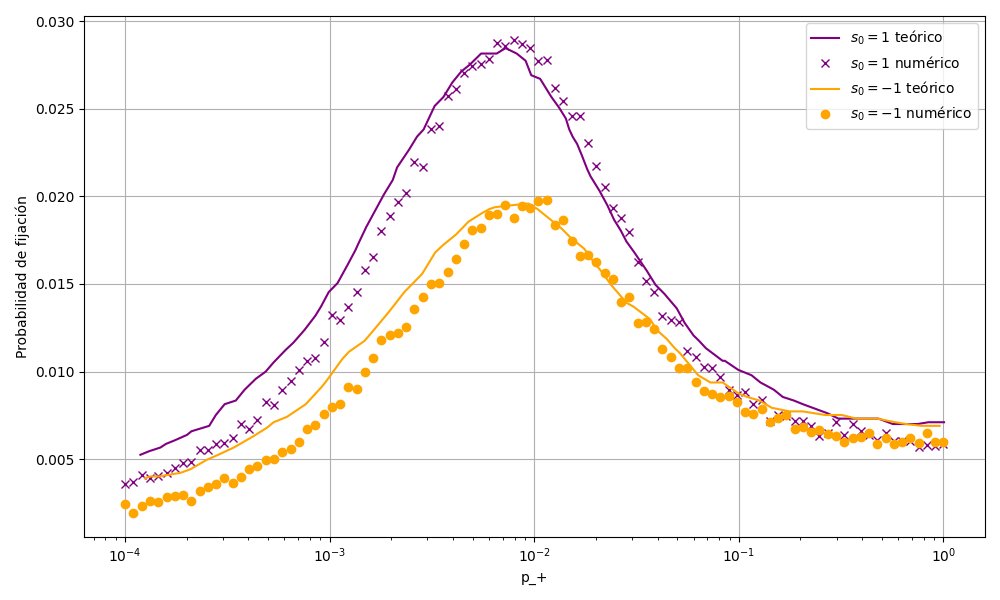
\includegraphics[width=\linewidth, height=4.5cm]{pronfijpmas.png} \\[2pt]
        \small a)
    \end{minipage}
    \hfill
    \begin{minipage}[t]{0.48\textwidth}
        \centering
        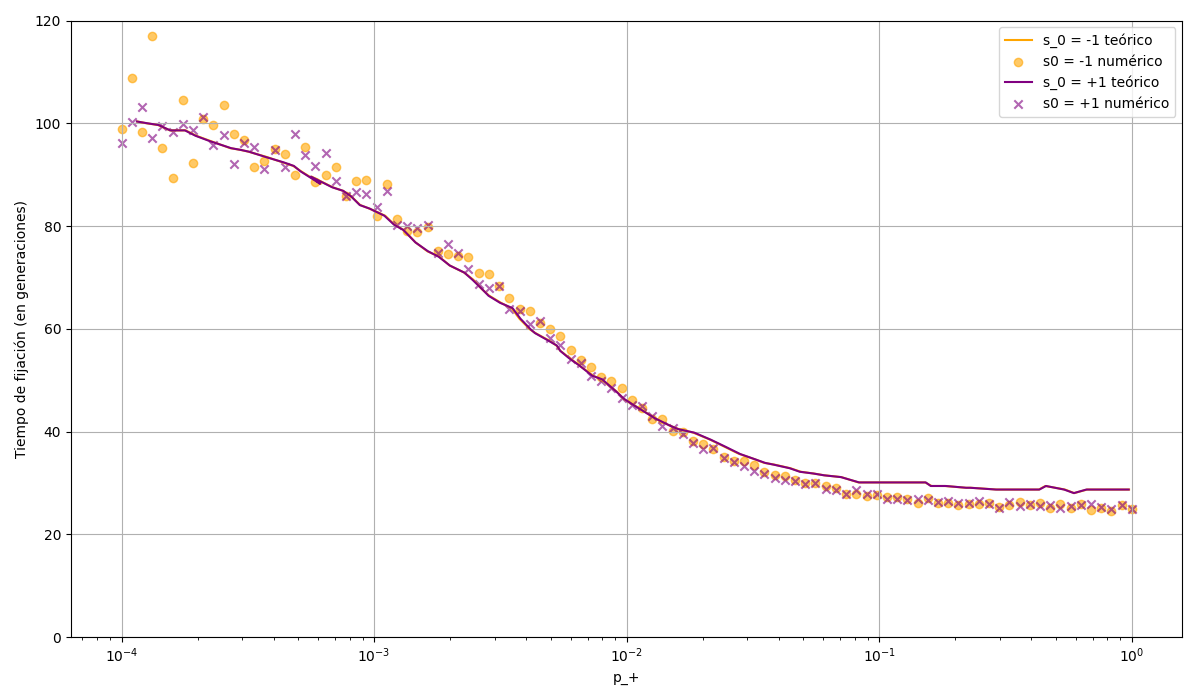
\includegraphics[width=\linewidth, height=4.5cm]{tiempofijgen.png} \\[2pt]
        \small b)
    \end{minipage}

    \caption{a) Probabilidad de fijación de un mutante en función de $p_+$ para dos ambientes iniciales distintos ($\sigma \pm 1$) con $p_- = 0.01$. Se muestran los resultados de simulación y teóricos descritos en el Apéndice  \ref{teoria ambiente}.
    b) Tiempo medio de fijación (en generaciones, i.e., N procesos de Moran) de un mutante en función de $p_+$ para dos ambientes iniciales distintos con $p_- = 0.01$. Se muestran los resultados de simulación y teóricos descritos en el Apéndice  \ref{teoria ambiente}. Los valores de la simulación se han obtenido generando trayectorias del proceso muerte-nacimiento usando el algoritmo de Gillespie. La matriz de pagos es $a_\sigma = d_\sigma = 1$, $b_\sigma = 1 + 0.5\sigma$ y $c_\sigma = 1 + 0.9\sigma$,  el tamaño del sistema es \( N = 50 \) y la intensidad de selección \( \beta = 0.5 \). Los resultados se han promediado mediante $10^5$ realizaciones. Se ha dejado pasar un tiempo suficiente de generaciones (máximo $10^5$).
    }


    \label{probfijytempfij}
\end{figure}


\subsection{Selección neutral bajo el límite de fast switching}

Procedemos a analizar un caso particular de matriz de pagos bajo el contexto del límite de fast switching. Este límite modela situaciones donde las interacciones entre agentes cambian rápidamente en comparación con la escala temporal de la evolución de estrategias.

Consideramos la siguiente matriz de pagos y su comportamiento determinista utilizando la dinámica del replicador, \cite{Ruben}.

\begin{equation}
M =
\begin{bmatrix}
b & b \\
1 & 1
\end{bmatrix}
\end{equation}

Se sustituye cada coeficiente en la ecuación del replicador \(\dot{x}=x(1-x)[(a-b-c+d)x+(b-d)]\) obteniendo \(\dot{x}=x(1-x)[(b-1)]\). Para los puntos fijos distinguimos entre los siguientes casos, \cite{CalvoTema2}.

\begin{itemize}
    \item $b=1$ tal que todos los puntos en $[0,1]$ son puntos fijos y por tanto no hay presión evolutiva que favorezca una estrategia sobre otra, siendo selección neutral
    \item $b \neq 1$ tal que los puntos fijos son $x^*=0$ y $x^*=1$

    \begin{itemize}
        \item Para $x^*=0$: $f'(0)=b-1$\\
        Si $b>1 \Rightarrow f'(0) >0 \Rightarrow \text{Inestable}$\\
        Si $b<1 \Rightarrow f'(0) <0 \Rightarrow \text{Estable}$\\
        \item Para $x^*=1$: $f'(1)=-b+1$\\
        Si $b>1 \Rightarrow f'(1) <0 \Rightarrow \text{Estable}$\\
        Si $b<1 \Rightarrow f'(1) >0 \Rightarrow \text{Inestable}$\\
    \end{itemize}
\end{itemize}

\begin{figure}[H]
  \centering
  \subfloat[b=1.5]{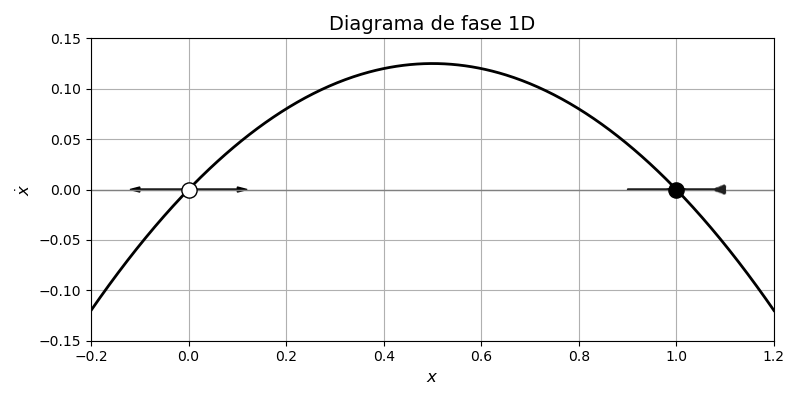
\includegraphics[width=0.47\textwidth]{Diagrama1.5.png}}
  \hspace{0.2cm}
  \subfloat[b=0.5]{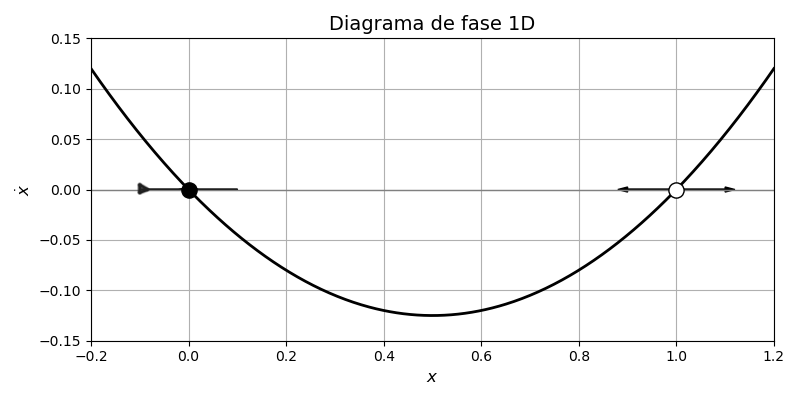
\includegraphics[width=0.47\textwidth]{Diagrama0.5.png}}
  \caption{Diagramas de fase unidimensionales para la dinámica replicadora \(\dot{x} = x(1-x)(b-1)\) con diferentes valores del parámetro \(b\). Los puntos fijos en \(x=0\) y \(x=1\) están indicados con círculos negros (estable) o blancos (inestable), y las flechas muestran la dirección del flujo. Se utilizó código en Python con librerías \texttt{numpy} y \texttt{matplotlib}.}
  \label{Diagramas} 
\end{figure}

En este caso, el jugador que sigue una estrategia $A$ tiene pago $p_A=b$ y el jugador que sigue una estrategia $B$ tiene pago $p_B=1$. Recurriendo al análisis de estabilidad podemos concluir que cuando $b>1 \Rightarrow p_A>p_B$ la población tiende a fijar la estrategia $A$ y cuando $b<1 \Rightarrow p_A<p_B$ tiende a fijar la estrategia $B$. El sistema experimenta una bifurcación transcrítica. Cuando $b>1$ hay dos puntos fijos, uno inestable y otro estable, cuando $b<1$ estos mismos puntos fijos intercambian estabilidad, ver Figura \ref{Diagramas}, \cite{CalvoTema2}.\\ 


Extendemos el análisis al caso en el que los valores \(b\) fluctúan aleatoriamente en cada paso de acuerdo a la distribución de probabilidad $f(b)$. Se define la probabilidad de transición efectiva como la esperanza de la probabilidad de transición:

\begin{equation}
T^{\pm}_{j,\mathrm{eff}} = \mathbb{E}[T^{\pm}_j] = \frac{j}{N} \cdot \frac{N - j}{N} \int \frac{1}{1 + \exp\left(\mp \beta \Delta \pi(b)\right)} f(b) \, db = \frac{j}{N} \cdot \frac{N - j}{N} I^{\pm}
\end{equation}

Con el razonamiento seguido en el Apéndice \ref{ApendiceC}, se concluye que como $I^-+I^+=1$, si asumimos $I^-=\frac{1}{2}$$ \Rightarrow I^+=\frac{1}{2}$. Entonces la probabilidad promedio de que $B$ reemplace a $A$ en un enfrentamiento directo es la misma de que $A$ reemplace a $B$. En otras palabras, ninguna estrategia tiene una ventaja evolutiva sobre la otra y por tanto el proceso es neutral en promedio, \cite{Ruben}.

La expresión de la línea de selección neutral bajo el límite de fast switching, siguiendo el Apéndice \ref{ApendiceC}, puede escribirse como:

\begin{equation}
    \mu = 1 -\sigma \sqrt{\frac{p_1}{p_2}} - \frac{1}{\beta}  ln f(\sigma)
\end{equation}

\subsection{¿Estrategias adversas al riesgo o estrategias propensas al riesgo?}

Tomando como propiedades primitivas en el estudio de la probabilidad de fijación el pago promedio del mutante ($\mu$) y la varianza del pago ($\sigma^2$), nos preguntamos en qué condiciones le conviene al mutante “jugar a lo seguro” —adoptar una estrategia con menor varianza (i.e., ser un generalista y optar por todos los ambientes)— o “apostar” —adoptar una estrategia con mayor varianza (i.e., ser un especialista y optar por el ambiente favorable aunque este sea raro). Aunque pueda parecer que la mejor opción es aumentar el pago medio ignorando la varianza, en \cite{DANINO201884} se introduce un parámetro de ruido en el sentido de una constante de difusión (esta se puede entender como una una varianza del entorno y puede ser vista como el riesgo asumido por el mutante en nuestra simulación) se concluye que las fluctuaciones ambientales pueden inducir una ventaja para estrategias de mayor varianza, incluso cuando estas tiene un pago medio menor.\newline



\begin{figure}[H]
    \centering
    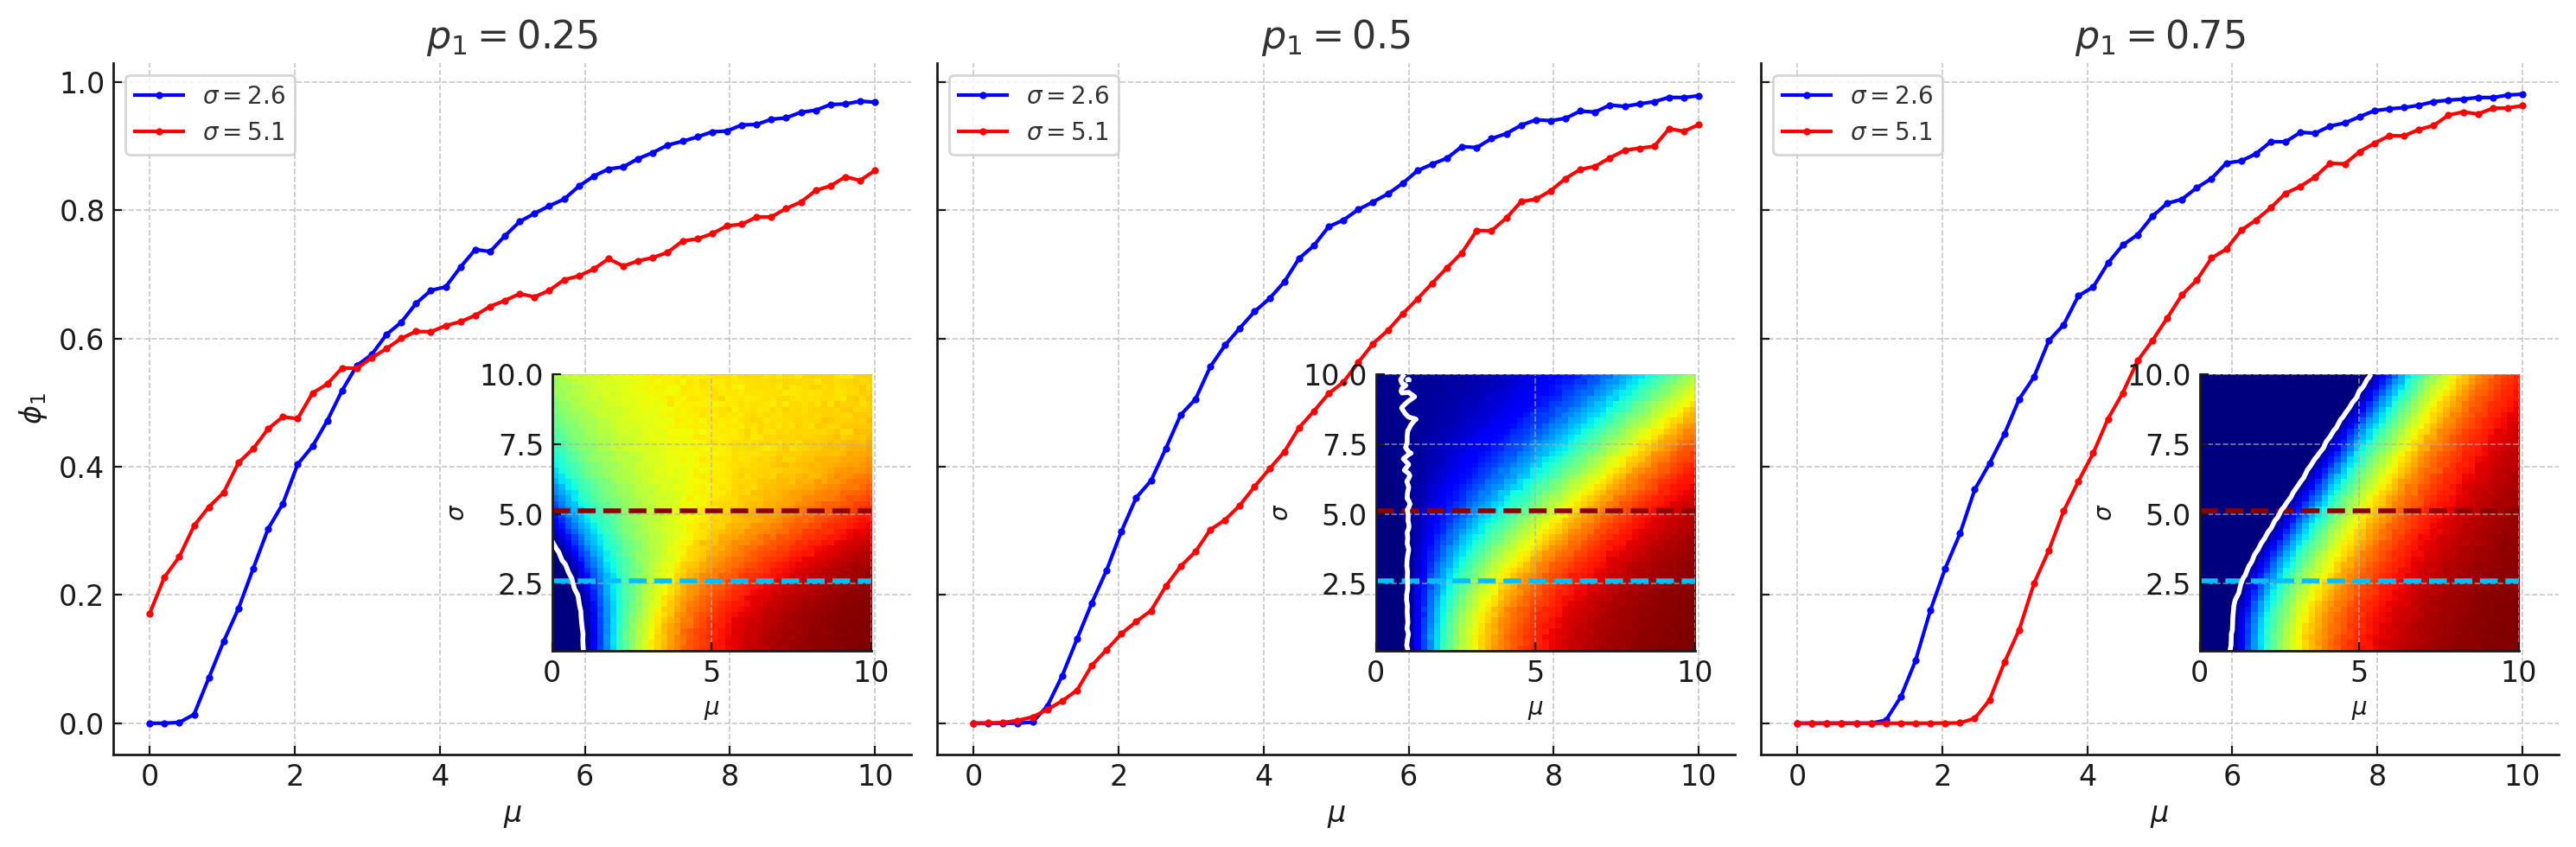
\includegraphics[width=1\linewidth]{figura15.png}
    \caption{ Probabilidad de fijación en función del valor medio del pago del mutante $\mu$ para $\sigma = 5.1$ (rojo) y $\sigma = 2.6$ (azul). Esto corresponde a los dos cortes mostrados en los recuadros inferiores derechos donde la linea blanca es la linea de selección neutral (la probabilidad de fijación es igual a 1/N). La escala va desde azul (probabilidad de fijación cercana a 0) a rojo (probabilidad de fijación cercana a 1). Se ha simulado una población de tamaño $N = 50$ con una intensidad de selección $\beta = 0.5$ tomando el límite de cambio rápido. Los datos son promediados sobre $ 10^{5}$ realizaciones dejando pasar un máximo de $10^5$ generaciones.}
    \label{fig15}
\end{figure}


En la Figura \ref{fig15} el mapa de calor en la gráfica izquierda, correspondiente a $p_1 = 0.25$ y $p_2 = 0.75$, muestra que la línea de selección neutral (probabilidad de fijación $\phi_1 = \frac{1}{N}$) está inclinada hacia la izquierda. Un mutante con una mayor varianza en la recompensa y una media más baja puede tener mayor probabilidad de fijación que un mutante con una mayor media de recompensa y menor varianza: se puede  ``apostar''.
Si la media es la misma para ambas estrategias se puede observar en las extracciones para $\sigma = 2,6$ y $\sigma = 5,1$ que la táctica con mayor varianza tiene mayor probabilidad de fijación solo hasta cierto valor de la media: antes de ese punto la apuesta es segura, a partir de tal punto es mejor para el mutante ``jugar a lo seguro'' y reducir la varianza.

El mapa de calor de la figura central ($p_1 = p_2 = 0.5$), la línea neutra es vertical. La única forma de alcanzar una probabilidad de fijación mayor a la neutra es aumentando la media. 
En las extracciones se observa que la estrategia con menor varianza obtiene mayor probabilidad de fijación: es mejor ``jugar a lo seguro''.

En mapa derecho ($p_1 = 0.75$, $p_2 = 0.25$), la línea de selección neutra se inclina hacia la derecha, de modo que un mutante con una menor media y menor varianza tiene más probabilidad de fijación que un mutante con una mayor media y mayor varianza: es mejor ``jugar a lo seguro''.


El caso de cambio rápido solo nos permite distinguir dos regímenes: apostar o jugar a lo seguro. Sin embargo, si en vez de considerar el fast switching limit analizamos el caso general donde el ambiente cambia con cierta probabilidad se puede especificar el tipo de apuesta. \newline


\begin{figure}[H]
    \centering
    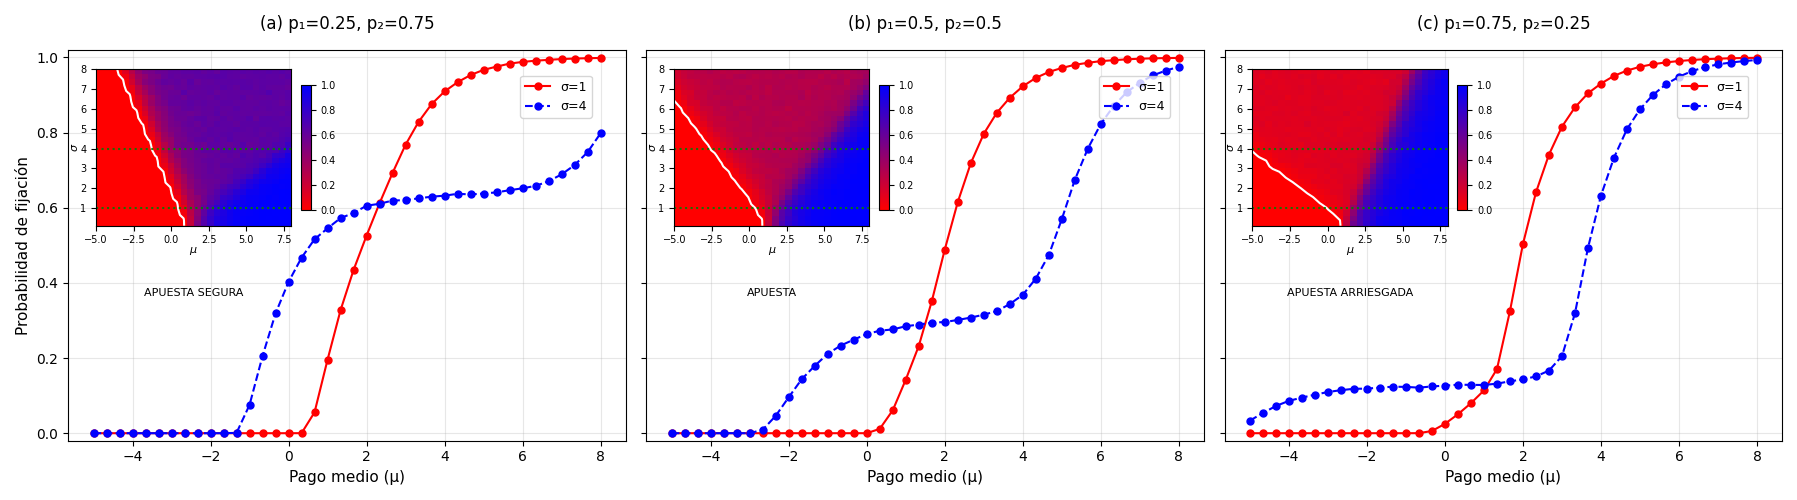
\includegraphics[width=1\linewidth]{figuraruben.png}
    \caption{ Probabilidad de fijación de un mutante para distribuciones de pago $p_1 = 0.25$, $0.5$ y $0.75$. 
    Los figuras principales muestran la probabilidad de fijación en función del pago medio del mutante $\mu$ para $\sigma = 1$ y $\sigma = 4$. Esto corresponde a los dos cortes mostrados en los recuadros superiores izquierdos donde la linea blanca es la linea de selección neutral (la probabilidad de fijación es igual a 1/N). La escala va desde azul (probabilidad de fijación cercana a 0) a rojo (probabilidad de fijación cercana a 1).
    Se simuló una población de tamaño $N = 50$ con intensidad de selección $\beta = 1$. Las probabilidades de cambio ambiental son $p^+ = 0.1/N$, $p^- = 0.1/(3N)$ en a), $p^+ = p^- = 0.1/N$ en b) y $p^+ = 0.1/(3N)$, $p^- = 0.1/N$ en c). Los datos se promediaron sobre $10^5$ realizaciones donde en cada realización el ambiente incial se eligió con probabilidad $p_1$ para $\sigma_0 = +1$ y $p_2$ para $\sigma_0 = -1$, además, se dejo pasar un tiempo suficientemente grande de generaciones ( máximo $10^5$).
    }
    \label{figuraruben}
\end{figure}



En la Figura \ref{figuraruben} se puede observar la probabilidad de fijación en función del pago medio del mutante ($\mu$) para distintas probabilidades de transición ambiental: en a) el entorno más favorable es el estado más probable, en b) los dos estados son equiprobables y en c) el entorno desfavorable es el más probable.


Cuando el pago del mutante es menor en promedio que el residente ($\mu < 0$) las estrategias con mayor varianza (riesgo) obtienen una mayor probabilidad de fijación: la apuesta es segura. El mutante puede especializarse en el ambiente favorable aunque suponga menor rendimiento en el ambiente desfavorable: el mutante puede aumentar su varianza aunque reduzca su media.
Aunque esto solo es posible cuando los cambios ambientales son lo suficientemente lentos para permitir que el mutante especializado absorba la población antes del cambio al ambiente desfavorable. En el caso c), donde el ambiente desfavorable es más probable, se nota que aumentar la varianza no implica una ventaja tan significativa como en el caso a): la apuesta es arriesgada.
En la Figura \ref{figuraruben} se puede observar que la diferencia de fijación entre ambas estrategias no es tan elevada como en a).

Estrategias de ``jugar a lo seguro'' (adversas a la varianza) son ventajosas para el mutante cuando su pago medio es mayor al del residente ($\mu > 0$): reducir parte de su pago medio a cambio de un menor sufrimiento ante el cambio ambiental lo convierte en un generalista.


\section{Dinámica tumoral}
\label{cancer}

Los tumores representan un ejemplo de la aplicación directa de la teoría de juegos, ya que las células cancerosas han perdido su comportamiento cooperativo normal y desertan. Sin embargo, resultados indican que los tumores no consisten en su totalidad de células cancerosas, lo cual plantea la posibilidad de que los quistes no sean el resultado de una mezcla aleatoria, sino que constituyan un equilibrio debido a las interacciones entre las células tumorales y normales \cite{Gerstung2011}. \\

 En su estudio sobre el mieloma múltiple (MM), un tipo de cáncer de la médula ósea, \cite{Pacheco2014} analizan, desde el enfoque de la teoría de juegos evolutiva, el equilibrio del remodelado óseo, determinado por la interacción entre la resorción ósea —llevada a cabo por los osteoclastos (OC)— y la formación ósea —realizada por los osteoblastos (OB). En nuestro marco, esto se modela como un juego de coexistencia, representado por una matriz de pagos:

\[
\begin{array}{c|cc}
     & \text{OC} & \text{OB} \\
\hline
\text{OC} & 0 & \alpha \\
\text{OB} & \varepsilon & 0 \\
\end{array}
\]

Donde $\varepsilon$ y $\alpha$ son números reales positivos. Lo que lleva a una ecuación del replicador: $\dot{x} = x(1-x)[\alpha(1-x) - \varepsilon x]$. Donde $x$ representa la fracción de células OC y $(1-x)$ la fracción de células OB. Dicha ecuación tiene puntos fijos en $x^* = 0$, $x^* = 1$ y $x^* = \alpha/(\alpha+\varepsilon)$. Los puntos $x^*=0$ y $x^*=1$ son puntos fijos inestables, mientras que $x^*=\alpha/(\alpha+\varepsilon)$ es estable, mostrando un equilibrio dinámico saludable.

Sin embargo, la aparición de células MM altera este equilibrio dinámico entre OB y OC a favor de los OC, ya que las MM segregan componentes químicos precursores de las OC. Además, las células OC también estimulan el crecimiento de la probación MM y estas últimas segregan proteínas que impiden la creación de nuevas células OB. Esta compleja interacción se puede describir  a través de la matriz de pagos:



\[
\begin{array}{c|ccc}
      & \text{OC} & \text{OB} & \text{MM} \\
\hline
\text{OC} & 0 & 1 & \beta \\
\text{OB} & 1 & 0 & -\delta \\
\text{MM} & \beta & 0 & 0 \\
\end{array}
\]


Donde las interacciones entre las células del mismo tipo son neutrales y los términos dentro de la matriz indican tasas de producción de distintos biocomponentes.
Dada esta interacción Pacheco et al. obtienen la Figura \ref{triangulos}. Los vértices de los triangulos indican poblaciones de un solo tipo celular, las aristas ausencia de al menos un tipo y el interior coexistencia de los tres tipos.

\begin{figure}[H]
    \centering
    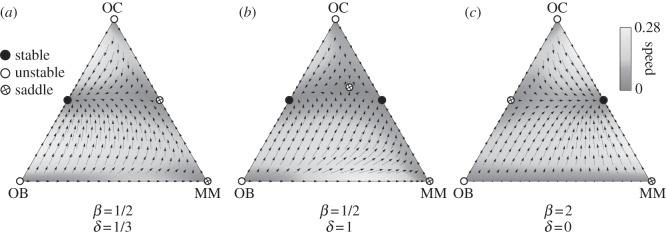
\includegraphics[width=0.55\linewidth]{triangulos cancer.jpg}
    \caption{Dinámica evolutiva de OC, OB y MM.
    a) Si $\beta < 1$: Las células MM pueden extinguirse, restableciéndose el equilibrio OB-OC. b) Si $\beta < 1$ pero $\beta + \delta > 1$, aparece un punto de silla que permite la coexistencia como posible estado final. c) Si $\beta > 1$, el único equilibrio estable es la coexistencia de MM y OC, llevando a destrucción ósea.
    Imagen tomada de \cite{Pacheco2014}.
    }
    \label{triangulos}
\end{figure}


Desde un punto de vista médico terapias que reduzcan $\beta$ disminuyen lesiones y ralentizan la progresión del cáncer, mientras que fármacos que actúen reduciendo $\delta$ mejoran la masa ósea y reducen el número de células cancerígenas.





%----------------------------------------------------------------------





\section{Conclusiones}




Este trabajo ha explorado cómo la teoría de juegos evolutivos puede servir como un marco riguroso para conectar modelos matemáticos con fenómenos biológicos observables. Las ecuaciones desarrolladas no son únicamente instrumentos de análisis cuantitativo, sino que formalizan principios evolutivos relevantes en distintos campos de la biología, desde interacciones moleculares hasta dinámicas poblacionales y ecológicas.

El análisis de ambientes fluctuantes ha permitido identificar una dinámica evolutiva no trivial: la adaptabilidad óptima no se alcanza en condiciones de estabilidad completa ni de variabilidad extrema, sino en regímenes intermedios. Esta observación, expresada en la relación entre los parámetros $p^+$, $p^-$ y las probabilidades de fijación, plantea una revisión de la aptitud biológica, al destacar su dependencia respecto del entorno fluctuante.

Adoptar estrategias de alta varianza (apostar) o de baja varianza (jugar a lo seguro) depende de las condiciones ambientales y del pago medio relativo al residente. Cuando el mutante presenta un pago medio inferior (\(\mu < 0\)), apostar —es decir, especializarse en el ambiente favorable a pesar de sufrir en el desfavorable— puede conferirle una ventaja en probabilidad de fijación, siempre que los cambios ambientales sean lo suficientemente lentos como para capitalizar el entorno favorable. En cambio, cuando el pago medio es superior (\(\mu > 0\)), reducir la varianza se torna ventajoso, permitiendo al mutante minimizar el impacto negativo de los cambios ambientales y consolidar su presencia en la población.


La aplicación de la teoría de juegos evolutivos a la dinámica tumoral, particularmente en el caso del mieloma múltiple, demuestra cómo cambios en la estructura de las interacciones celulares pueden inducir transiciones entre regímenes evolutivos de coexistencia y coordinación. Este enfoque permite reinterpretar la progresión del cáncer como una alteración del equilibrio poblacional, impulsada por parámetros como $\beta$ y $\delta$, y sugiere que terapias efectivas podrían orientarse a modificar dichas interacciones en lugar de atacar directamente a las células tumorales.



Finalmente, el marco desarrollado ofrece implicaciones relevantes en distintas áreas de investigación. En oncología, sugiere enfoques terapéuticos basados en la modificación del microambiente tumoral más que en intervenciones directas sobre las células cancerosas. En ecología, aporta herramientas para modelar la viabilidad de especies invasoras bajo condiciones ambientales no estacionarias. Y en biología evolutiva, establece un vínculo formal entre la teoría de juegos y los modelos dinámicos no lineales. En conjunto, este estudio contribuye a una visión más integrada de la evolución, donde los modelos matemáticos permiten descripciones de sistemas biológicos complejos.
 























%--------------------------------------------------------------------

\newpage

\renewcommand{\appendixname}{Apéndice}
\appendix
\section{Derivación de expresiones para la fijación estocástica} 
\label{ApendiceA}

\subsection{Derivación de la probabilidad de fijación de un mutante, \cite{Arne}}
\vspace{0,2 cm}

Se calcula la probabilidad de fijación de un mutante,para un estado intermedio se utiliza una ecuación de balance teniendo en cuenta todas las posibles transiciones en el siguiente paso \(\phi_j=T_j^+\phi_{j+1}+T_j^-\phi_{j-1}+(1-T_j^+-T_j^-)\phi_j \)\\

Se reescribe la ecuación de balance:

\[
0=-T_j^-(\phi_j-\phi_{_{j-1}})+T_j^+(\phi_{j+1}-\phi_j)
\]

Se define la variable \(y_j=\phi_{j}-\phi_{j-1}\) que representa la diferencia entre probabilidades de fijación en estados consecutivos:

\[
0=T_j^+y_{j+1}-T_j^-y_j \Rightarrow y_{j+1}=\frac{T_j^-}{T_j^+}y_j=\xi_j y_j
\]

Se usa la relación recursiva \(y_{j+1}=\xi_j y_j\) teniendo en cuenta que en los estados absorbentes \(\phi_0=0,\phi_N=1\): \(y_1=\phi_1-\phi_0=\phi_1,y_2=\phi_2-\phi_1=\xi_1 y_1=\xi_1 \phi_1,y_3=\phi_3-\phi_2=\xi_2y_2=\xi_2 \xi_1\phi_1...\) y se llega a la siguiente expresión:

\[
y_k=\phi_k-\phi_{k-1}=\phi_1 \prod_{j=1}^{k-1} \xi_j
\]

Nota: No se define \(\xi_0\) porque no tiene sentido físico, no hay individuos que usen la estrategia \(A\).\\

Para aislar $\phi_1$ y obtener una fórmula explícita para la probabilidad de fijación de un mutante se suman todos los \(y_k\) de $1$ hasta $N$ tal que \(\sum_{k=1}^{N}y_k=(\phi_1-\phi_0)+(\phi_2-\phi_1)+...+(\phi_N-\phi_{N-1})=\phi_N-\phi_0=1-0=1\) (suma telescópica), sustituyendo en la anterior expresión:

\[
\sum_{k=1}^{N}y_k=\sum_{k=1}^{N}\phi_1 \prod_{j=1}^{k-1} \xi_j=1 
\]

Si \(k=1\) se tiene un producto vacío pues no hay ningún \(j\) que cumpla \(1 \leq j \leq 0\), por convención matemática el producto vacío es igual a la unidad tal que \(\prod_{j=1}^{0}\xi_j=1\).Se despeja \(\phi_1\) definiendo una nueva variable \(m=k-1\):

\[
\sum_{k=1}^{N} \phi_1 \prod_{j=1}^{k-1} \xi_j=\phi_1+\sum_{k=2}^{N} \phi_1 \prod_{j=1}^{k-1}\xi_j=\phi_1\left(1+\sum_{m=1}^{N-1}\prod_{j=1}^{m}\xi_j \right)=1  \Rightarrow \phi_1=\frac{1}{\left(1+\sum_{m=1}^{N-1}\prod_{j=1}^{m}\xi_j \right)}
\]

\subsection{Derivación del tiempo de fijación de un mutante, \cite{Arne}}

Se calcula el tiempo de fijación de un mutante,para un estado intermedio se utiliza una ecuación de balance  teniendo en cuenta todas las posibles transiciones en el siguiente paso,  por convención matemática se suma \(1\) ya que ese paso ya consume una unidad de tiempo: \( t_j=T_j^+t_{j+1}+T_j^-t_{j-1}+(1-T_j^+-T_j^-)t_j +1\)\\ 

Se reescribe la ecuación de balance:

\[
0=-T_j^-(t_j-t_{_{j-1}})+T_j^+(t_{j+1}-t_j)+1
\]

Se define la variable \(z_j=t_{j}-t_{j-1}\) que representa la diferencia entre tiempos de fijación en estados consecutivos:

\[
0=T_j^+z_{j+1}-T_j^-z_j +1\Rightarrow z_{j+1}=\frac{T_j^-}{T_j^+}z_j-\frac{1}{T_j^+}=\xi_j z_j-\frac{1}{T_j^+}
\]

Se usa la relación recursiva \(z_{j+1}=\xi_j z_j-\frac{1}{T_j^+}\) teniendo en cuenta que en los estados absorbentes \(t_0=0,t_N=0\): \(z_1=t_1-t_0=t_1,z_2=t_2-t_1=\xi_1 z_1-\frac{1}{T_1^+}=\xi_1 t_1-\frac{1}{T_1^+},z_3=t_3-t_2=\xi_2z_2-\frac{1}{T_2^+}=\xi_2 \left(\xi_1t_1-\frac{1}{T_1^+}\right)-\frac{1}{T_2^+}...\) y se llega a la siguiente expresión:

\[
z_k=t_k-t_{k-1}=t_1 \prod_{m=1}^{k-1} \xi_m-\sum_{l=1}^{k-1}\frac{1}{T_l^+}\prod_{m=l+1}^{k-1}\xi_m
\]


Para aislar $t_1$ y obtener una fórmula explícita para el tiempo de fijación de un mutante se suman todos los \(z_k\) de $j+1$ hasta $N$ tal que \(\sum_{k=j+1}^{N}z_k=(t_{j+1}-t_j)+(t_{j+2}-t_{j+1})+...+(t_N-t_{N-1})=t_N-t_j=0-t_j=-t_j\), partiendo de \(-t_1=\sum_{k=2}^{N}z_k\) se expande la suma definiendo una nueva variable \(w=k-1\):


\[
t_1=-\sum_{k=2}^{N}z_k=-\sum_{k=2}^{N} \left( t_1 \prod_{m=1}^{k-1} \xi_m-\sum_{l=1}^{k-1}\frac{1}{T_l^+}\prod_{m=l+1}^{k-1}\xi_m \right)=-t_1\sum_{k=2}^{N}\prod_{m=1}^{k-1} \xi_m+\sum_{k=2}^{N}\sum_{l=1}^{k-1}\frac{1}{T_l^+}\prod_{m=l+1}^{k-1}\xi_m 
\]

\[
t_1=-t_1\sum_{w=1}^{N-1}\prod_{m=1}^{w} \xi_m+\sum_{w=1}^{N-1}\sum_{l=1}^{w}\frac{1}{T_l^+}\prod_{m=l+1}^{w}\xi_m \Rightarrow t_1\left(1+ \sum_{w=1}^{N-1}\prod_{m=1}^{w} \xi_m \right)=\sum_{w=1}^{N-1}\sum_{l=1}^{w}\frac{1}{T_l^+}\prod_{m=l+1}^{w}\xi_m 
\]

\[
t_1=\frac{\sum_{w=1}^{N-1}\sum_{l=1}^{w}\frac{1}{T_l^+}\prod_{m=l+1}^{w}\xi_m}{\left(1+ \sum_{w=1}^{N-1}\prod_{m=1}^{w} \xi_m \right)}=\phi_1 \left( \sum_{w=1}^{N-1}\sum_{l=1}^{w}\frac{1}{T_l^+}\prod_{m=l+1}^{w}\xi_m \right )
\]

\hspace{0,5 cm}

\section{Derivación de expresiones para la dinámica nacimiento-muerte} 
\label{ApendiceB}

\subsection{Derivación de la ecuación de Langevin, \cite{CalvoTema3}}

Se considera una dinámica de nacimiento-muerte, se calcula la probabilidad de tener \(j\) individuos en un tiempo \(t+\Delta t\):

\[
P(j;t+\Delta t)=T_{j-1}^+P(j-1;t)+T_{j+1}^-P(j+1;t)+(1-T_{j}^+-T_{j}^-)P(j;t)
\] 


Se realiza una expansión de Kramers-Moyal, se calcula el paso mínimo que puede dar \(x\) tal que \(\Delta x=x_{j+1}-x_j=\frac{j+1}{N}-\frac{j}{N}=\frac{1}{N}\):

\[
P(x;t+\Delta t)=T_{x-\Delta x}^+P(x-\Delta x;t)+T_{x+\Delta x}^-P(x+ \Delta x;t)+(1-T_{x}^+-T_{x}^-)P(x;t)
\] 

Si \(N>>1\) y \(x\) es continua entonces se puede realizar una expansión de taylor de una función compuesta \(f_{x\pm h}\cdot P(x \pm h;t)=T_x \cdot P(x;t)\pm\partial_x(T_x \cdot P(x;t)) \cdot h+ \frac{1}{2} \partial_x^2 (T_x \cdot P(x;t)) \cdot h^2+O(h^3)\):

\[
P(x;t+\Delta t)=-\partial_x(T_x^+P(x;t))\frac{1}{N}+\frac{1}{2}\partial_x^2(T_x^+P(x;t))\frac{1}{N^2}+\partial_x(T_x^-P(x;t))\frac{1}{N}+\frac{1}{2}\partial_x^2(T_x^-P(x;t))\frac{1}{N^2}+P(x;t)
\]

\[
P(x;t+\Delta t)-P(x;t)=-\frac{\partial_x}{N}((T_x^+-T_x^-)P(x;t))+\frac{\partial_x^2}{2N^2}((T_x^++T_x^-)P(x;t))
\]

Se utiliza la definición de derivada parcial temporal \(\frac{\partial f(x;t)}{\partial t} = \lim_{\Delta t \to 0} \frac{f(x; t + \Delta t) - f(x; t)}{\Delta t}\), se divide por \(\Delta t\) y se toma el límite \(\Delta t \xrightarrow{} 0\):

\[
\partial_tP(x;t)=-\text{lim}_{\Delta t \xrightarrow{}0}\frac{h}{\Delta t}\partial_x((T_x^+-T_x^-)P(x;t))+\text{lim}_{\Delta t \xrightarrow{}0} \frac{h^2}{2 \Delta t}\partial^2_x((T_x^++T_x^-)P(x;t))
\]

Para que los coeficientes de las parciales no se anulen y no diverjan se utiliza \(\Delta t \sim h\):

\[
\partial_tP(x;t)=-\partial_x((T_x^+-T_x^-)P(x;t))+ \frac{1}{2 N}\partial^2_x((T_x^++T_x^-)P(x;t))=-\partial_x(A(x)P(x;t))+\frac{1}{2}\partial^2_x(B(x)P(x;t))
\]

Se considera la ecuación de Langevin asociada a esta Fokker-Planck, considerando el término de deriva \(A(x)\) y el término de difusión \(B(x)\):

\[
\dot{x}(t)=A(x)+\sqrt{B(x)} \xi(t) \Rightarrow \dot{x}(t)=(T_x^+-T_x^-)+\sqrt{\frac{(T_x^++T_x^-)}{N}}\xi(t)
\]


\subsection{Derivación de la ecuación del replicador ajustada, \cite{CalvoTema3}}

Se toma el límite \(N \xrightarrow{ }\infty\) para recuperar la dinámica replicadora ajustada:

\[
\dot{x}(t)=(T_x^+-T_x^-)=x(1-x) \left(\frac{1}{1+\text{exp}(- w \Delta \pi(x))}  -\frac{1}{1+\text{exp}(+w \Delta \pi(x))}\right)=x(1-x)\left( \frac{\text{exp}(+w \Delta \pi(x))-1}{\text{exp}(+w \Delta \pi(x))+1}\right) 
\]

Se utiliza la identidad de la tangente hiperbólica \(\text{tanh}(x/2)=\frac{e^{x/2}-e^{-x/2}}{e^{x/2}+e^{-x/2}}=\frac{e^x-1}{e^x+1}\):

\[
\dot{x}(t)=x(1-x)\text{tanh}(+\frac{w}{2} \Delta \pi(x))=x(1-x)\text{tanh}(+\frac{w}{2} (\pi_A(x)-\pi_B(x))))
\]




%--------------------------------------------------------------------

\section{Derivación de expresiones para la probabilidad de fijación y tiempo de fijación en el caso de ambiente cambiante}
\label{teoria ambiente}

\cite{Ashcroft2014} proponen una teoría lineal en la que la probabilidad de fijación y tiempo de fijación se calculan de forma recursiva.

La probabilidad de fijación obedece las condiciones de contorno $\phi_{0,\sigma} = 0$ y $\phi_{N,\sigma} = 1 $ y la relación:

\[
\phi_{j,\sigma} = \sum_{i=1}^{j} \left[ \frac{1-p_{-\sigma} }{\Delta} \nu_{i, \sigma} - \frac{p_\sigma}{\Delta} \nu_{i, -\sigma} \right]
\]



Donde $\Delta$ es el determinante de la matriz de pagos del respectivo ambiente y los términos $\nu_{j, \sigma}$ se extraen de forma recursiva usando la ligadura $\sum_{i=1}^{j} \nu_j = 1$ y la relación:

\[
    \nu_{j+1, \sigma} = \gamma_{j, \sigma} \nu_{j, \sigma} + \frac{1}{\omega^+_{j, \sigma}} \frac{p_\sigma}{\Delta} \sum_{i=1}^{j} (\nu_{i, \sigma} - \nu_{i, -\sigma})
\]

Donde $\gamma_{j, \sigma} = \frac{\omega^-_{j, \sigma}}{\omega^+_{j, \sigma}}$.

Por su parte el tiempo de fijación condicionado al mutante (tipo A) se extrae utilizando las condiciones de contorno $t_{0,\sigma} = t_{N,\sigma} = 0 $ y la relación: 

\[
    t^A_{j, \sigma} = \frac{1}{\phi_{j, \sigma}} \sum_{i=1}^{j} \left[ \frac{1 - p_{-\sigma}}{\Delta} \eta_{i, \sigma} - \frac{p_\sigma}{\Delta} \eta_{i, -\sigma} \right]
\]

Donde:

\[
    \eta_{j+1, \sigma} = \gamma_{j, \sigma} \nu_{j, \sigma} + \frac{1}{\omega^+_{j, \sigma}} \frac{p_\sigma}{\Delta} \sum_{i=1}^{j} (\eta_{i, \sigma} - \eta_{i, -\sigma}) - \frac{1}{\omega^+_{j, \sigma}} \phi_{j, \sigma}
\]



\section{Derivación de expresiones para la dinámica bajo el límite de fast switching}
\label{ApendiceC}
\subsection{Derivación de la condición de selección neutral, \cite{Ruben}}

Se define la línea de selección neutral como el conjunto de parámetros ($\mu,\sigma$) tales que la probabilidad de fijación de un mutante es $\phi=1/N$, se recupera así la definición de probabilidad clásica si ninguna estrategia tiene ventaja evolutiva sobre la otra, es decir, \(T_{j,eff}^-=T_{j,eff}^+\). Formalmente esto se describe así:

\[
    \phi_1=\frac{1}{1+\sum_{k=1}^{N-1}\prod_{j=1}^{k} \xi_j} , \xi_j=\frac{T_j^-}{T_j^+} \Rightarrow \phi_1=\frac{1}{N}
\]

\vspace{0,2 cm}
Por un lado se suman los términos \(I^+\) y \(I^-\):

\[
I^- + I^+ = \int f(b) \left[ \frac{1}{1 + e^{\beta (b-1)}} + \frac{1}{1 + e^{-\beta (b-1)}} \right] db = \int f(b)\, db = 1 
\]

Donde se ha utilizado que la distribución de probabilidad está normalizada y que \(\frac{1}{1 + e^{x}} + \frac{1}{1 + e^{-x}}=\frac{1}{1 + e^{x}} + \frac{1}{\frac{1+e^x}{e^x}} =\frac{1 + e^{x}}{1 + e^{x}}=1\).

\vspace{0,2 cm}

Por otro lado, por definición \(\frac{T_{j,eff}^-}{T_{j,eff}^+}=\frac{I^-}{I^+}\) puesto que se cancelan los términos \(\frac{j}{N} \cdot \frac{N - j}{N}\). Si es selección neutral entonces \(\frac{T_{j,eff}^-}{T_{j,eff}^+}=\frac{I^-}{I^+}=1 \Rightarrow I^-=I^+\). 

\vspace{0,4 cm}
Finalmente, dado que \(I^-+I^+=1\) y \(I^-=I^+\), se llega a \(2I^-=1\Rightarrow I^-=\frac{1}{2}\)

\subsection{Derivación de la expresión de selección neutral, \cite{Ruben}}

Partiendo de la condición $I^- = \frac{1}{2}$ derivada en la sección anterior para el caso de selección neutral se obtiene:

\[
    I^- = \int \frac{1}{1 + \exp\left(- \beta \Delta \pi(b)\right)} f(b) \, db = \frac{1}{2}
\]

En el límite de cambio rápido el mutante \textit{siente} una media ponderada de ambos ambientes. De esta forma se puede considerar $f(b)$ como
una distribución de probabilidad discreta que toma dos valores $b_1$ y $b_2$. Donde el mutante \textit{siente} de media cada pago pesado por su probabilidad $p_1$ y $p_2$ respectivamente, obteniendo la relación:

\[
    \frac{p_1}{1 + \exp\left(- \beta (b_1 -1)\right)} + \frac{p_2}{1 + \exp\left(- \beta (b_2 -1)\right)} = \frac{1}{2}
\]

Además, $f(b)$ tiene media $\mu = b_1p_1 + b_2p_2$ y varianza $\sigma^2 = (b_1 - \mu)^2p_1 + (b_2 - \mu)^2p_2$. Así, se pueden expresar los parámetros como: $b_1 = \mu - \sigma \cdot \sqrt{ \frac{p_2}{p_1} },
b_2 = \mu + \sigma \cdot \sqrt{ \frac{p_1}{p_2} }$. Y la relación anterior toma la forma:

\[
 \frac{p_1}{1 + \exp\left(-\beta \left[ \mu - \sigma \cdot \sqrt{\frac{p_2}{p_1}} -1 \right] \right)} + 
\frac{p_2}{1 + \exp\left(-\beta \left[ \mu + \sigma \cdot \sqrt{\frac{p_1}{p_2}} -1 \right] \right)} = \frac{1}{2}
\]

Expresión de cual no es trivial hallar una forma funcional para $\mu$. Por ello, dado que tenemos una expresión del tipo $f(\mu, \sigma) = cte$ hacemos el siguiente ansatz $\mu = 1 -\sigma \sqrt{\frac{p_1}{p_2}} - \frac{1}{\beta}  ln f(\sigma)$, obteniendo:

\[
f(\sigma) = \left( p_1 - \frac{1}{2} \right) \left( \frac{1}{\gamma(\sigma)} - 1 \right)
+ \frac{1}{2\gamma(\sigma)} 
\sqrt{4(\gamma(\sigma) - 1)^2 p_1 (1 - p_1) + (\gamma(\sigma) + 1)^2}
\]

Donde \( \gamma(\sigma) \) es:

\[
\gamma(\sigma) = \exp\left[
\beta \sigma \left( 
\sqrt{ \frac{p_1}{1 - p_1} } + \sqrt{ \frac{1 - p_1}{p_1} }
\right)
\right]
\]


\nocite{*}
\bibliography{sorsamp}% Produces the bibliography via BibTeX.

\end{document}
%
% ****** End of file sorsamp.tex ******

